%-------------------------------------------------------------
% Language
% Use the option "language=EN" to set the beamer theme in English. Use
% the option "language=ES" to set the beamer theme in Spanish.

% Colors
% Use the option "color=white" to set the background in white and the
% bottom bar in blue. Use the option "color=blue" to set the
% background in blue and the bottom bar in white. Use the option
% "color=blue2" to set the background in blue and the bottom bar in
% blue.

% Font Color
% Use the option "fontc=black" to set the font color in black. If this
% argument is not given the default color is set depending of the
% color scheme selected.

% Notes:
% Do not use \large inside multicols
% Enumerate require \justifying command
% Tables captions bellow the tabular
% With citations, note = {} may only work for @misc

% Credits: https://github.com/alejogm0520 & Samuel Plazas Escudero
%-------------------------------------------------------------

%--Principal packages
\documentclass[xcolor=table, aspectratio=43,8pt]{beamer} % 4:3; can be 16:9; [...,8pt,t] in order to start text of all frames on the upper part; add: draft to not compile figures.
\usetheme[language=ES, color=white]{EAFIT}
\usepackage[spanish]{babel}
\decimalpoint % All decimal numbers with point
\usepackage[utf8]{inputenc}
\selectlanguage{spanish}
\usepackage{amsmath,amsfonts,amssymb,cancel} % Equations; physics is optional and sometimes problematic!
\usepackage{verbatim} % Environments, \begin{comment}
%--Arial
\usepackage{helvet}\renewcommand{\familydefault}{\sfdefault} % It's ok
%--David Plazas recommended
%\usepackage{libertine} % Normal
%--Carlos Cuartas 
%\usepackage[T1]{fontenc}\usepackage{lmodern} % Best
%--Beamer packages
\usepackage{tikz} % For making vectorized figures, arrows
\usepackage{ifthen} % For specifying conditionals for sections
\usepackage{ragged2e}\justifying % Whole text justified, except enumerate: add \justifying
\usepackage{multicol} % Multiple columns in one frame
%--Tables-Figures

\renewcommand\spanishtablename{Tabla}
\usepackage{booktabs,multirow} % Bookstyle tables
\usepackage{array} % Custom width and centered
\newcolumntype{P}[1]{>{\centering\arraybackslash}p{#1}} % horizontal centering but use custom width
\newcolumntype{M}[1]{>{\centering\arraybackslash}m{#1}} % horizontal and vertical centering but use custom width
%-Figure label
\usepackage[labelsep=period,justification=justified,format=plain]{caption} % Dot instead of colon and justified caption
%--Figure
\usepackage{graphicx,subcaption} % Figures and subfigures
\usepackage{media9} % video and audio
%-Figure-Table on top
\usepackage{float} % Allows to put H instead of ht
\setbeamertemplate{caption}[numbered] % Numbered captions
%---------TOC
\setbeamertemplate{section in toc}[sections numbered]
\setbeamertemplate{subsection in toc}[subsections numbered]
\setbeamerfont{section in toc}{size=\small}
\setbeamerfont{subsection in toc}{size=\footnotesize}
\setbeamertemplate{subsection in toc}{\leavevmode\leftskip=3.2em\rlap{\hskip-2em\inserttocsectionnumber.\inserttocsubsectionnumber}\inserttocsubsection\par} % Indented subsection
\setcounter{tocdepth}{2} % Toc depth, put 1 for only showing there the sections and 2 to include sections
%---------Cite
\usepackage{bibentry} % Full cite foot
\nobibliography* % Full cite foot
\setbeamertemplate{bibliography item}[triangle]% [online][book][article][triangle][text]; Or: \setbeamertemplate{bibliography item}{\insertbiblabel} 
\usepackage{etoolbox} % Package for using justified bibliography 
\apptocmd{\thebibliography}{\justifying}{}{} % Justified bibliography 
%---------Footnotes
\setbeamercolor{footnote}{fg=white} % Footnote white 
\setbeamercolor{footnote mark}{fg=.} % Takes the color depending on the circumpstance
\setbeamercolor{bibliography entry author}{fg=white} % Allows to have white footnote bibs
\setbeamertemplate{footnote}
{
  \hspace*{-1cm} % Horizontal movement
  \vspace*{-3.12cm} % Vertical movement
  \parbox[c][3.64cm]{10.6cm}{\tiny\noindent\insertfootnotemark\insertfootnotetext} % b: bottom, height: 3.3cm, horizontal length: 10.6cm (max horizontal)
% If there are problems, put \vspace*{-2.87cm} and \parbox[c][3.3cm]
% or \vspace*{-2.88cm} and \parbox[c][3.4cm]
% or \vspace*{-3.05cm} and \parbox[c][3.6cm]
% or \vspace*{-3.12cm} and \parbox[c][3.64cm]
}
\renewcommand{\footnoterule}{\kern -3pt \hrule width \textwidth height 0pt\kern 3pt} % No footnoterule
\usepackage{perpage}\MakePerPage{footnote} % Footnote numbered per frame
\renewcommand{\thefootnote}{\Roman{footnote}} % Roman number in footnote
                                              % Cutom: \fnsymbol{footnote}
%------------------------------------
%---------Numbered Slides and Sections
\setbox0=\hbox{\subsecname\unskip}\ifdim\wd0=0pt\else%
 ~--~\insertsubsectionhead
\fi
%------Numbering section: title in bold, centered and with a line
\newcommand{\numb} 
{
  \setbeamertemplate{frametitle}
  {
    \ifx\insertsubsection\empty % No subsection
         \bfseries\thesection.~\insertframetitle~\color{black}\par\vskip-5pt\hrulefill % \centering
    \else % subsection
         \bfseries\thesection.~\insertframetitle~\color{black}\par\vskip-9pt\hrulefill\par\vskip3pt{\large\thesection.\thesubsection~\insertframesubtitle} % Subsection with smaller size;
    \fi
  }
}
%------No numbering section: title in bold, centered and with a line
\newcommand{\nonumb}
{
  \setbeamertemplate{frametitle}{\bfseries\color{black}\centering\insertframetitle\par\vskip-6pt\hrulefill}
}
%------------------------------------
%--No hyphenation on text
\tolerance=1
\emergencystretch=\maxdimen
\hyphenpenalty=10000
\hbadness=10000
%------------------------
%---------Itemize justified in beamer
\makeatletter
\renewcommand{\itemize}[1][]{
  \beamer@ifempty{#1}{}{\def\beamer@defaultospec{#1}}
  \ifnum \@itemdepth >2\relax\@toodeep\else
    \advance\@itemdepth\@ne
    \beamer@computepref\@itemdepth % Sets \beameritemnestingprefix
    \usebeamerfont{itemize/enumerate \beameritemnestingprefix body}
    \usebeamercolor[fg]{itemize/enumerate \beameritemnestingprefix body}
    \usebeamertemplate{itemize/enumerate \beameritemnestingprefix body begin}
    \list
      {\usebeamertemplate{itemize \beameritemnestingprefix item}}
      {\def\makelabel##1{
          {
            \hss\llap{{
                \usebeamerfont*{itemize \beameritemnestingprefix item}
                \usebeamercolor[fg]{itemize \beameritemnestingprefix item}##1}}
          }
        }
      }
  \fi
  \beamer@cramped
  \justifying % Justified itemize
  \beamer@firstlineitemizeunskip
}
\makeatother
%------------------------
%---------get current section name for showing it at its begining
\usepackage{nameref}
\makeatletter
\newcommand*{\currentname}{\@currentlabelname}
\makeatother
%---------Shows in which section we are at the begining of each one
%\begin{comment}
\AtBeginSection[]
{
\begin{frame}[plain,noframenumbering]
  \begin{beamercolorbox}[ht=\paperheight,wd=\paperwidth, center]{Portada}
    \begin{center}\textbf{\LARGE \currentname}\end{center} % Leave the next space mandatorily

    \vspace{0.44\paperheight}
  \end{beamercolorbox}
\end{frame}
}
%\end{comment}

%-------------------(CONSTANTLY BEING EDITED)------------------
%---------TEXTBLOCKS-GRID 
\usepackage[absolute,overlay,showboxes]{textpos}
%\usepackage[texcoord,grid,gridunit=mm,gridcolor=red!10,subgridcolor=green!10]{eso-pic} % Helping grids, comment when publishing
%---------NOTES IN BEAMER
\AtBeginNote{\Huge}\newcommand{\notei}[1]{\note[item]{\Huge{\textcolor{blue}{#1}}}} % Use \notei{text} everywhere % [1] means one parameter located in #1 (input). 
\setbeamertemplate{note page}[plain] % Plain style for notes page
\setbeameroption{show notes} % {show notes} or {hide notes}
% \setbeameroption{show notes on second screen=right}
% as well you can use \documentclass[notes=only] at the beginning of the code
%-----------More elaborated notes
%\setbeamercolor{note page}{bg=white!90!black, fg=black}
%\setbeamercolor{note title}{bg=white!30!red, fg=black}
%\setbeamercolor{note date}{parent=note title}
%---------Itemize, enumberate and lists inside them
%\setbeamertemplate{itemize/enumerate body begin}{\LARGE} % Body
\setbeamertemplate{itemize/enumerate subbody begin}{\Large} % Subbody
%---------COLOR DEFINITIONS
\definecolor{azure(colorwheel)}{rgb}{0.0, 0.5, 1.0} % Define colors here
\definecolor{blue(ryb)}{rgb}{0.01, 0.28, 1.0}
\graphicspath{{figs/}}
\usepackage[normalem]{ulem}
\useunder{\uline}{\ul}{}

%%%%%%%%%%%%%%%%%%%%%%%
%Start of the Document%
%%%%%%%%%%%%%%%%%%%%%%%

%---------COVER PAGE
  \title{ANÁLISIS DE VARIANZA DE UN SOLO\\ \vspace{2.5mm}FACTOR PARA \boldmath{$K\geq2$}}
\author{\normalfont\texorpdfstring{Presentado por:\\Mateo Restrepo S.\\Juan S. Cárdenas R. \\David Plazas E.\\[1ex]Prof.: Francisco I. Zuluaga}{}}

\def\carrera{Ingeniería Matemática}
\def\departamento{Departamento de Ciencias Matemáticas}
\def\escuela{Escuela de Ciencias}
\def\eafit{Universidad EAFIT}
\def\materia{Estadística I}
\def\fecha{2018} % or put the exact date
% to add more def, search for "Dirección" in beamerthemeEAFIT.sty

%\includeonly{Slides/0_cover_title,ex_beamer,Slides/refs_thanks}
\begin{document}
\nonumb % Not numbered titles
\begin{frame}
% Portada Inspira Crea Transforma
\end{frame}
%%%%%%%%%%%%%%%%%%%%%%%%%%%%%%%%%%%%%%%%%%%%%%%%%%%%%%%%%%%%%%%%%%%%%%%%%%%%
\begin{frame}
\begin{center}
  \titlepage % Cover page
\end{center}
\end{frame}
%%%%%%%%%%%%%%%%%%%%%%%%%%%%%%%%%%%%%%%%%%%%%%%%%%%%%%%%%%%%%%%%%%%%%%%%%%%%
\begin{frame}{CONTENIDO}
\begin{multicols}{2}
  \tableofcontents
\end{multicols}
\end{frame}
\numb % Numbered titles
%\begin{comment}
\section{DESCRIPCIÓN DE LA PRUEBA}
\begin{frame}{DESCRIPCIÓN DE LA PRUEBA}
\begin{itemize}
    \item La idea es determinar si hay diferencias significativas entre las medias de las poblaciones, comparando sus varianzas. Este método es una generalización de la \textit{prueba-t} de dos muestras, estudiado en clase \footnote{\bibentry{stat}}.
    \item Sea $k$ el número de poblaciones a ser analizadas, donde $Y_{ij}$ es la j-ésima unidad experimental para la i-ésima muestra, donde $i=1,...,k$ y $j=1,...,n_i$, donde $n_i$ es el tamaño de la i-ésima muestra.
    \item \textbf{Suposiciones:} Si el tamaño de la muestra es pequeño (i.e $n<30$), se debe suponer que la población sigue una distribución normal. Además, se supone que las poblaciones son independientes (tanto en muestras grandes como pequeñas) con medias $\mu_1,\mu_2,...,\mu_k$ y varianzas $\sigma_1^2=\sigma_2^2=...=\sigma_k^2=\sigma^2$.
    
    %La idea es hallar un estimador insesgado para $\sigma$.
\end{itemize}
\end{frame}
\subsection{Prueba de hipótesis}
\begin{frame}{DESCRIPCIÓN DE LA PRUEBA}
    \framesubtitle{Prueba de hipótesis}
    Basados en las pruebas ya mostradas, se requiere construir una prueba de hipótesis para determinar si existe evidencia suficiente para afirmar que $\mu_1=\mu_2=...=\mu_k$\footnote{\bibentry{stat}}.\vspace{2mm}
    
    \textbf{Hipótesis nula\\}
    $H_0:\quad\mu_1=\mu_2=...=\mu_k$
    \vspace{2mm}
    
    \textbf{Hipótesis alterna\\}
    $H_1:\quad(\exists\hspace{1mm} i,j)(\mu_i\ne\mu_j)\rightarrow$ Si al menos una de las igualdades no se cumple.\vspace{2mm}
    
    \begin{multicols}{2}
    \textbf{Estadístico de prueba\\}
    \[F=\dfrac{SST\Big/k-1}{SSE\Big/n-k}\sim\mathbb{F}_{(k-1,n-k)}\quad\text{, bajo } H_0\]
    \textbf{Región de Rechazo}
        \[RR:\left\{F>F_\alpha\right\}\]
        \columnbreak
        \begin{figure}[H]
            \centering
            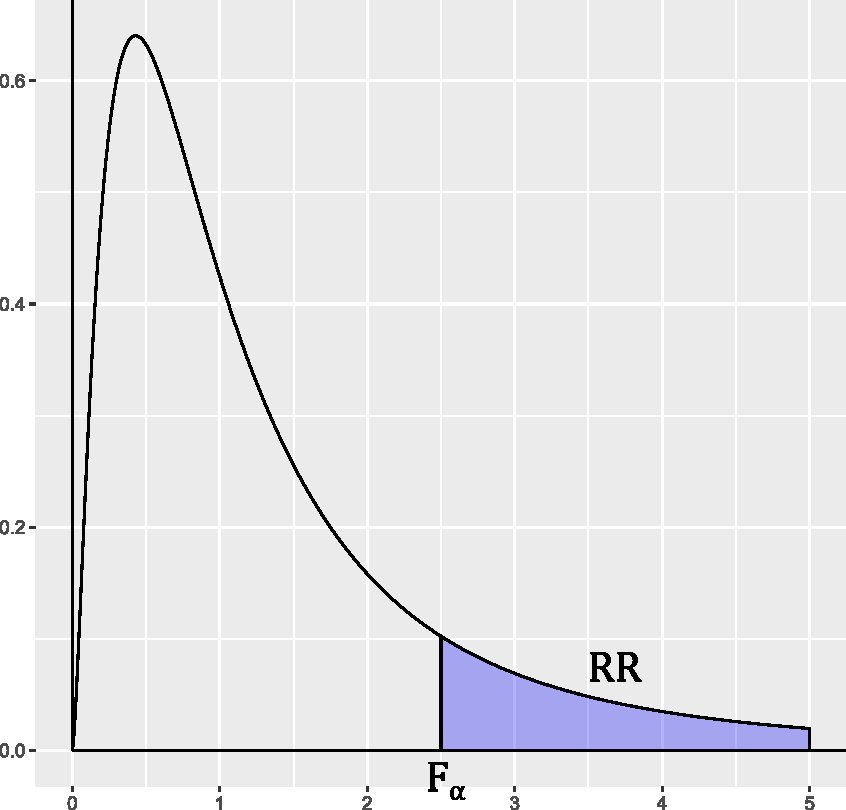
\includegraphics[width=45mm, height=35mm]{F.pdf}
        \end{figure}
    \end{multicols}
\end{frame}
\subsection{Preliminares}
\begin{frame}{DESCRIPCIÓN DE LA PRUEBA}
\framesubtitle{Preliminares}

    \begin{equation*}
        Y_i=\sum_{j=1}^{n_i}Y_{ij} \qquad E\left(Y_i\right)=n_i\mu_i \qquad V\left(Y_i\right)=n_i\sigma^2
    \end{equation*}
    \begin{equation*}
        \Bar{Y_i}=\dfrac{1}{n_i}Y_i \qquad E\left(\Bar{Y_i}\right)=\mu_i \qquad V\left(\Bar{Y_i}\right)=\dfrac{\sigma^2}{n_i}
    \end{equation*}
    \begin{equation*}
        \Bar{Y}=\dfrac{1}{n}\sum_{i=1}^kn_i\Bar{Y}_i\qquad\text{SST}=\sum_{i=1}^{k}\dfrac{Y_i^2}{n_i}-n\Bar{Y}^2\qquad \text{SSE}=\sum_{i=1}^{k}\sum_{j=1}^{n_i}\left(Y_{ij}-\Bar{Y}_i\right)^2
    \end{equation*}
    Se utilizarán estas variables aleatorias, con sus respectivas medias y varianzas, para calcular la esperanza del SST\footnote{\bibentry{stat}} (Total sum of squares), utilizando
    \begin{equation*}
        E\left(Y^2\right)=V(Y)+E^2\left(Y\right)
    \end{equation*}
        
    
\end{frame}

\begin{frame}{DESCRIPCIÓN DE LA PRUEBA}
\framesubtitle{Preliminares}
\begin{equation*}
\begin{split}
    E(SST)&=E\left(\sum_{i=1}^k\dfrac{Y_i^2}{n_i}\right)-E(n\Bar{Y}^2)\\
    &=\sum_{i=1}^k\dfrac{E\left(Y_i^2\right)}{n_i}-nE(\Bar{Y}^2)\\
    &=\sum_{i=1}^k\dfrac{n_i\sigma^2+(n_i\mu_i)^2}{n_i}-n\left(\dfrac{\sigma^2}{n}+\dfrac{1}{n^2}\left(\sum_{i=1}^kn_i\mu_i\right)^2\right)\\
    &=\sum_{i=1}^k\left(\sigma^2+n_i\mu_i^2\right)-\sigma^2-\dfrac{1}{n}\left(\sum_{i=1}^kn_i\mu_i\right)^2\\
    &=(k-1)\sigma^2+\sum_{i=1}^kn_i\mu_i^2-\dfrac{1}{n}\left(\sum_{i=1}^kn_i\mu_i\right)^2
\end{split}
\end{equation*}
\end{frame}

\begin{frame}{DESCRIPCIÓN DE LA PRUEBA}
\framesubtitle{Preliminares}
En el caso de $\mu_1=\mu_2=...=\mu_k=\mu$\footnote{\bibentry{stat}}, 
\begin{equation*}
    \begin{split}
        E(SST)&=(k-1)\sigma^2+\sum_{i=1}^kn_i\mu^2-\dfrac{1}{n}\left(\sum_{i=1}^kn_i\mu\right)^2\\
        &=(k-1)\sigma^2+\mu^2\sum_{i=1}^kn_i-\dfrac{\mu^2}{n}\left(\sum_{i=1}^kn_i\right)^2\\
        &=(k-1)\sigma^2+n\mu^2-n\mu^2
    \end{split}
\end{equation*}
    \begin{equation}
        E\left(\dfrac{SST}{k-1}\right)=\sigma^2
    \end{equation}
    Nótese que $\dfrac{SST}{k-1}$ es un estimador insesgado de $\sigma^2$. Siguiendo un procedimiento análogo, se puede probar que $\dfrac{SSE}{n-k}$ es otro estimador insesgado para $\sigma^2$.
\end{frame}


    
\section{FORTALEZAS Y DEBILIDADES}
\begin{frame}{FORTALEZAS Y DEBILIDADES\footnote{\bibentry{stat}}}
\begin{multicols}{2}
\textbf{Fortalezas}
\begin{itemize}
    \item No importan los tamaños de las muestras o si no son iguales.
    \item Permite encontrar dos estimadores insesgados para $\sigma^2$.
    \item Permite tener en cuenta cuantas muestras se desee.
    \item Permite hallar (o no) evidencia suficiente para verificar si $\mu_1=\mu_2=...=\mu_k$.
\end{itemize}
\columnbreak
\textbf{Debilidades}
\begin{itemize}
    \item Se debe suponer normalidad en las poblaciones ($n<30$).
    \item Se debe suponer que las varianzas poblacionales para todas las muestras deben ser iguales.
    \item Se debe comprobar primero que las muestras sean independientes (podrían utilizarse métodos como el test de Levene\footnote{\bibentry{levene}}).
\end{itemize}
\end{multicols}
\end{frame}
\section{EJEMPLOS}
\subsection{Para 4 muestras}
\begin{frame}{EJEMPLOS}
    \framesubtitle{Para 4 muestras\footnote{\bibentry{stat}}}
    
    Cuatro grupos de estudiantes se someten a diferentes técnicas de enseñanza y se examinan al final de un periodo especificado. Como consecuencia de las deserciones de los grupos experimentales (por enfermedad, transferencia, etc.), el número de estudiantes varió de un grupo a otro. ¿Los datos mostrados en la Tabla \ref{tab:ejem1} presentan suficiente evidencia para indicar una diferencia en el éxito medio para las cuatro técnicas de enseñanza?
    
    \begin{table}[H]
        \begin{tabular}{ccccc}
        \hline
                    & 1      & 2      & 3        & 4     \\ \hline
                    & 65     & 75     & {\ul 59} & 94    \\
                    & 87     & 69     & 78       & 89    \\
        {\ul }      & 73     & 83     & 67       & 80    \\
                    & 79     & 81     & 62       & 88    \\
                    & 81     & 72     & 83       &       \\
                    & 69     & 79     & 76       &       \\
                    &        & 90     &          &       \\ \hline
        $y_i$       & 454    & 549    & 425      & 351   \\
        $n_i$       & 6      & 7      & 6        & 4     \\
        $\Bar{y}_i$ & 75.667 & 78.429 & 70.833   & 87.750 \\ \hline
        \end{tabular}
        \caption{}
        \label{tab:ejem1}
    \end{table}
\end{frame}

\begin{frame}{EJEMPLOS}
    \framesubtitle{Para 4 muestras\footnote{\bibentry{stat}}}
    Para el estadístico de prueba, se requiere el SST y SSE:
    \begin{equation*}
        \begin{split} \text{SST}=&\sum_{i=1}^{k}\dfrac{Y_i^2}{n_i}-n\Bar{Y}^2\approx712.586 \\\text{SSE}=&\sum_{i=1}^{k}\sum_{j=1}^{n_i}\left(Y_{ij}-\Bar{Y}_i\right)^2\approx1196.631
        \end{split}
    \end{equation*}
    Por lo tanto,
    \begin{equation*}
        F=\dfrac{SST\Big/k-1}{SSE\Big/n-k}\approx3.771
    \end{equation*}
    
\end{frame}

\begin{frame}{EJEMPLO}
\framesubtitle{Para 4 muestras\footnote{\bibentry{stat}}}
    Para un nivel de significancia del 5\% (i.e. $\alpha=0.05$), se debe calcular $F_\alpha$. Utilizando el comando
    
    \begin{center}
    \texttt{F\_alpha <- qf(0.05, k-1, n-k, lower.tail = FALSE)}
    \end{center}
    
    Que retorna un valor de $F_\alpha\approx3.127$. Por lo tanto, la RR es
    \begin{equation*}
        RR:\left\{F>3.127\right\}
    \end{equation*}
    
    Como $3.771>3.127$, se puede rechazar $H_0$, ya que hay suficiente evidencia para afirmar esto; por lo tanto, existe una diferencia significativa entre las medias de las 4 poblaciones.
\end{frame}

\begin{frame}{EJEMPLOS}
    \framesubtitle{Para 4 muestras\footnote{\bibentry{stat}}}
    Este resultado también se puede comprobar con el $valor-p$ ($V_p$); como se rechazó $H_0$, el $V_p$ debería ser menor o igual al nivel de significancia de la prueba. Para esto, utilizamos los comandos
    
    \begin{center}
        \texttt{F <- (SST/(k-1))/(SSE/(n-k))\\
        p\_value <- pf(F, k-1, n-k, lower.tail = FALSE)}
    \end{center}
    
    Que resulta en $V_p\approx0.028$, que efectivamente es menor al nivel de la prueba ($\alpha=0.05$) y se comprueba que el resultado previo.
\end{frame}

\subsection{Para 2 muestras}
\begin{frame}{EJEMPLOS}
    \framesubtitle{Para 2 muestras\footnote{\bibentry{stat}}}
    Los valores codificados para una medida de elasticidad de un plástico preparado por dos procesos diferentes se proporcionan en la Tabla \ref{tab:ejem2}. Las muestras independientes, ambas de tamaño 6, se tomaron de la producción de cada uno de los procesos. ¿Los datos presentan suficiente evidencia para indicar una diferencia en elasticidad media en los dos procesos?
    \begin{table}[H]
        \begin{tabular}{ccc}
        \hline
                     & \textbf{A}    & \textbf{B}    \\ \hline
                     & 6.1  & 9.1  \\
                     & 7.1  & 8.2  \\
                     & 7.8  & 8.6  \\
                     & 6.9  & 6.9  \\
                     & 7.6  & 7.5  \\
                     & 8.2  & 7.9  \\ \hline
        $y_i$        & 43.7 & 48.2 \\
        $n_i$        & 6    & 6    \\
        $\Bar{y_i}$ & 7.28 & 8.03 \\ \hline
        \end{tabular}
        \caption{}
        \label{tab:ejem2}
    \end{table}
\end{frame}

\begin{frame}{EJEMPLOS}
\framesubtitle{Para 2 muestras\footnote{\bibentry{stat}}}
    Para el estadístico de prueba, se requiere el SST y SSE:
    \begin{equation*}
        \begin{split} \text{SST}=&\sum_{i=1}^{k}\dfrac{Y_i^2}{n_i}-n\Bar{Y}^2\approx1.688 \\\text{SSE}=&\sum_{i=1}^{k}\sum_{j=1}^{n_i}\left(Y_{ij}-\Bar{Y}_i\right)^2\approx 5.862
        \end{split}
    \end{equation*}
    Por lo tanto,
    \begin{equation*}
        F=\dfrac{SST\Big/k-1}{SSE\Big/n-k}\approx 2.879
    \end{equation*}
    
\end{frame}

\begin{frame}{EJEMPLO}
\framesubtitle{Para 2 muestras\footnote{\bibentry{stat}}}
    Para un nivel de significancia del 5\% (i.e. $\alpha=0.05$), se debe calcular $F_\alpha$. Utilizando el comando
    
    \begin{center}
    \texttt{F\_alpha <- qf(0.05, k-1, n-k, lower.tail = FALSE)}
    \end{center}
    
    Que retorna un valor de $F_\alpha\approx4.964$. Por lo tanto, la RR es
    \begin{equation*}
        RR:\left\{F>4.964\right\}
    \end{equation*}
    
    Como $2.879<4.964$, no se puede rechazar $H_0$, ya que no hay suficiente evidencia a favor de $H_1$; por lo tanto, no existe una diferencia significativa entre las medias de las 2 poblaciones.
\end{frame}

\begin{frame}{EJEMPLOS}
    \framesubtitle{Para 2 muestras\footnote{\bibentry{stat}}}
    Este resultado también se puede comprobar con el $valor-p$ ($V_p$); como se no rechazó $H_0$, el $V_p$ debería ser mayor al nivel de significancia de la prueba. Para esto, utilizamos los comandos
    
    \begin{center}
        \texttt{F <- (SST/(k-1))/(SSE/(n-k))\\
        p\_value <- pf(F, k-1, n-k, lower.tail = FALSE)}
    \end{center}
    
    Que resulta en $V_p\approx0.12$, que efectivamente es mayor al nivel de la prueba ($\alpha=0.05$) y se comprueba que el resultado previo.
\end{frame}

%\end{comment}
\nonumb % Not numbered titles
%\addcontentsline{toc}{section}{\small\protect\numberline{}{REFERENCIAS BIBLIOGRÁFICAS}} % Separated from other contents, for small number of contents
\addcontentsline{toc}{section}{\small REFERENCES} % Closer from other contents, for large number of contents
\nocite{*} % All citations showed (take care with fraud!)
%%%%%%%%%%%%%%%%%%%%%%%%%%%%%%%%%%%%%%%%%%%%%%%%%%%%%%%%%%%%%%%%%%%%%%%%%%%%
\section*{REFERENCES}
\begin{frame}[allowframebreaks]{REFERENCES} %  and put before {REFEREN...}
\begingroup % Group for changing the color
\renewcommand{\color}[1]{} % Allows to have black bibs and white footnote bibs
\small{\bibliographystyle{IEEEtran}} % Size of text; acm or gatech-thesis or ieeetr or ieeetran or icontec or iso690
\bibliography{ref}
\endgroup % Group for changing the color
% pdflatex -> bibtex -> pdflatex -> pdflatex
\end{frame}
%%%%%%%%%%%%%%%%%%%%%%%%%%%%%%%%%%%%%%%%%%%%%%%%%%%%%%%%%%%%%%%%%%%%%%%%%%%%
% Thank-slide
\begin{frame}[plain,noframenumbering] % No frame number
	\begin{beamercolorbox}[ht=\paperheight,wd=\paperwidth, center]{Portada}
		\begin{center}\Huge\textbf{Thank you}\end{center} % Or Thanks; leave the next space mandatorily
		
		\vspace{0.44\paperheight}
    \end{beamercolorbox}
\end{frame}
%%%%%%%%%%%%%%%%%%%%%%%%%%%%%%%%%%%%%%%%%%%%%%%%%%%%%%%%%%%%%%%%%%%%%%%%%%%%


\end{document}